\documentclass{fkssolpub}

\usepackage[czech]{babel}
\usepackage{fontspec}
\usepackage{fkssugar}
\usepackage{amsmath}
\usepackage{graphicx}

\author{Ondřej Sedláček}
\school{Gymnázium Oty Pavla} 
\series{2p}
\problem{2} 

\begin{document}

Proužek můžeme při pokrývání krychle přehýbat takto (vyšrafovaná část je otočena směrem ke středu krychle, přehyby jsou vyznačeny přerušovanými čarami):

\begin{figure}[h!]
	\begin{center}
		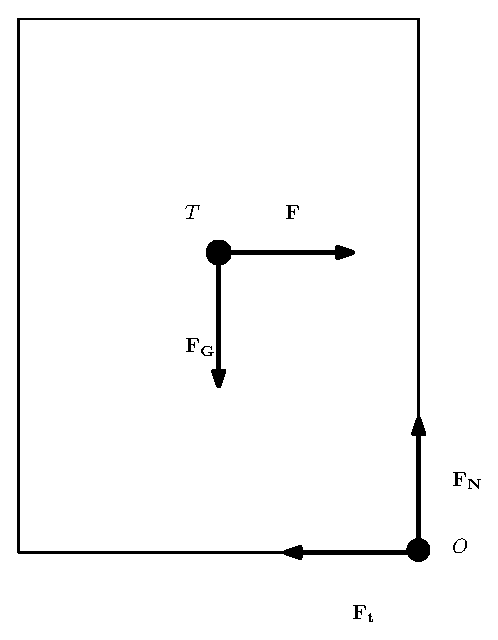
\includegraphics[width=0.95\textwidth]{2-fig}
	\end{center}
	\caption{Přehýbání proužku překrývající krychli}
	\label{fig:1}
\end{figure}


\end{document}
